\documentclass[10pt,a4paper]{amsart}
\usepackage{amsmath,amssymb,amsthm,graphicx}
\usepackage{amsmath,amssymb,graphicx,mathtools}
\newcommand{\by}[1]{\overset{\scriptscriptstyle #1}{=}}
\title{Laplace distributors correspond bijectively to exponential maps on the monoidal unit}
\author{Marie Kerjean, Jean-Simon Pacaud Lemay}
\date{doi:10.4230/LIPIcs.FSCD.2024.9; CC BY4.0 (official publisher paper)}
\begin{document}
\maketitle
\noindent\textit{Editorial note.} Source https://drops.dagstuhl.de/entities/document/10.4230/LIPIcs.FSCD.2024.9. © Marie Kerjean and Jean-Simon Pacaud Lemay, CC BY4.0. Statement and full author proof faithfully transcribed from the published PDF; original defining and proof diagrams retained.\par\medskip
\noindent\textit{Allowed standard prerequisites (editorial).}\begin{itemize}
\item Additive symmetric monoidal closed categories and monoidal differential coalgebra modalities. Publisher§2 and references[2],[18],[22]. Exact canonical-map equations(4)–(10) and the compatibility identities actually used in the proof are retained.
\end{itemize}\medskip
% BEGIN CONTEXT: publisher Sections2-3, pp9:5-9:8
\section*{Background: Differential Categories}
We follow the terminology and notation of the source.
The underlying categorical structure is an additive symmetric monoidal category.
We denote the underlying category by $\mathcal C$, the monoidal product by $\otimes$,
the monoidal unit by $I$, the natural associativity isomorphism by
$\alpha_{A,B,C}:A\otimes(B\otimes C)\to(A\otimes B)\otimes C$,
the natural right unital isomorphism by $\rho_A:A\otimes I\to A$,
and the natural symmetry isomorphism by $\sigma_{A,B}:A\otimes B\to B\otimes A$.
Each homset is a commutative monoid with addition $+$ and zero $0$, and composition
and $\otimes$ are compatible with the additive structure.

A coalgebra modality is a comonad $!$ with digging $p_A:!A\to!!A$ and
dereliction $d_A:!A\to A$, contraction $c_A:!A\to!A\otimes!A$ and
weakening $w_A:!A\to I$, making each $!A$ a cocommutative comonoid and
digging a comonoid morphism. A monoidal coalgebra modality furthermore has
$\mu_{A,B}:!A\otimes!B\to!(A\otimes B)$ and $\mu_I:I\to!I$ making
$!$ lax monoidal; $p,d,c,w$ are monoidal transformations, and $c,w$ are
$!$-coalgebra morphisms.
In the additive setting one obtains co-contraction
$\bar c_A:!A\otimes!A\to!A$ and co-weakening $\bar w_A:I\to!A$,
making each $!A$ a commutative monoid, and in fact a bimonoid.
A monoidal differential modality additionally has a co-dereliction
$\bar d_A:A\to!A$ with the differential-category axioms of source reference[2].
A differential linear category is an additive symmetric monoidal category with
a monoidal differential modality. A differential linear closed category is one
whose underlying symmetric monoidal category is closed.

We write $A\multimap B$ for internal homs and
$\epsilon_{A,B}:(A\multimap B)\otimes A\to B$ for evaluation.
For $f:C\otimes A\to B$, its unique curry $\lambda(f):C\to A\multimap B$ satisfies
\begin{equation}(\lambda(f)\otimes1_A);\epsilon_{A,B}=f.\tag{4}\end{equation}
Composition is diagrammatic: $f;g$ denotes first $f$, then $g$.
For $f:X\to A$ and $g:B\to Y$, the map
$f\multimap g:A\multimap B\to X\multimap Y$ is characterized by
\begin{equation}
((f\multimap g)\otimes1_X);\epsilon_{X,Y}
=(1_{A\multimap B}\otimes f);\epsilon_{A,B};g.\tag{5}
\end{equation}
For a monoidal coalgebra modality the canonical
$\xi_{A,B}:!(A\multimap B)\to!A\multimap!B$ satisfies
\begin{equation}
(\xi_{A,B}\otimes1_{!A});\epsilon_{!A,!B}
=\mu_{A\multimap B,A};!\epsilon_{A,B}.\tag{6}
\end{equation}
The dual object is $A^*=A\multimap I$; duality need not be involutive.
The canonical isomorphism $\upsilon_I:I\to I^*$ is characterized by
\begin{equation}
(\upsilon_I\otimes1_I);\epsilon_{I,I}=\rho_I,
\qquad \upsilon_I^{-1}=\rho_{I^*}^{-1};\epsilon_{I,I}.\tag{7}
\end{equation}
The canonical $\nu_{A,B}:(A\otimes B)^*\to A\multimap B^*$ and its inverse satisfy
\begin{align}
((\nu_{A,B}\otimes1_A)\otimes1_B);(\epsilon_{A,B^*}\otimes1_B);\epsilon_{B,I}
&=\alpha_{(A\otimes B)^*,A,B}^{-1};\epsilon_{A\otimes B,I},\notag\\
(\nu_{A,B}^{-1}\otimes1_{A\otimes B});\epsilon_{A\otimes B,I}
&=\alpha_{A\multimap B^*,A,B};(\epsilon_{A,B^*}\otimes1_B);\epsilon_{B,I}.\tag{8}
\end{align}
The canonical $\Theta_{A,B}:A^*\otimes B^*\to(A\otimes B)^*$ satisfies
\begin{equation}
(\Theta_{A,B}\otimes1_{A\otimes B});\epsilon_{A\otimes B,I}
=\tau_{A^*,B^*,A,B};(\epsilon_{A,I}\otimes\epsilon_{B,I});\rho_I,\tag{9}
\end{equation}
where $\tau$ swaps the middle two terms. For $f:A\to B$, duality gives
$f^*:B^*\to A^*$ characterized by
\begin{equation}
(f^*\otimes1_A);\epsilon_{A,I}=(1_{B^*}\otimes f);\epsilon_{B,I}.\tag{10}
\end{equation}

\paragraph{Definition1.}
For a differential linear closed category, a Laplace distributor is a natural
transformation $\ell_A:!A^*\to(!A)^*$ such that the following original
commutative diagrams hold:
\begin{center}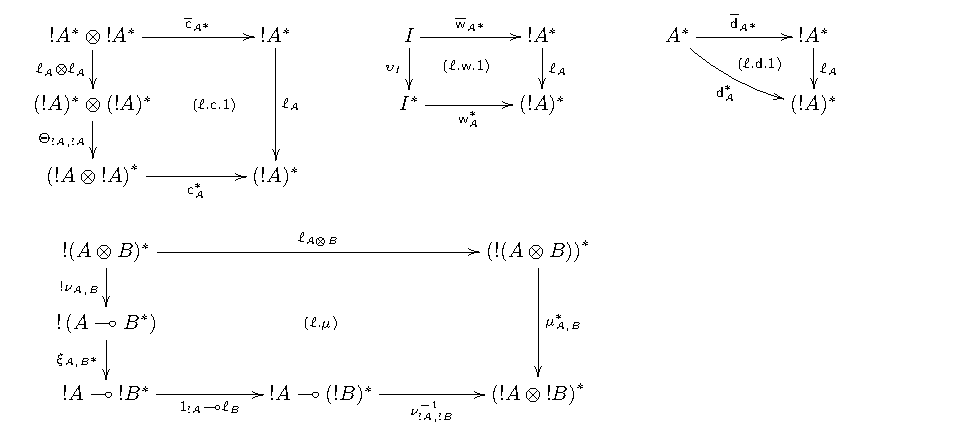
\includegraphics[width=\linewidth]{laplace-distributor-laws.pdf}\end{center}
These are the source axioms $(\ell.\bar c.1)$, $(\ell.\bar w.1)$,
$(\ell.\bar d.1)$ and $(\ell.\mu)$.
\paragraph{Definition2.}
The original definition of the Laplace evaluator and its extranaturality equation are retained here, including the author's evaluator glyph:
\begin{center}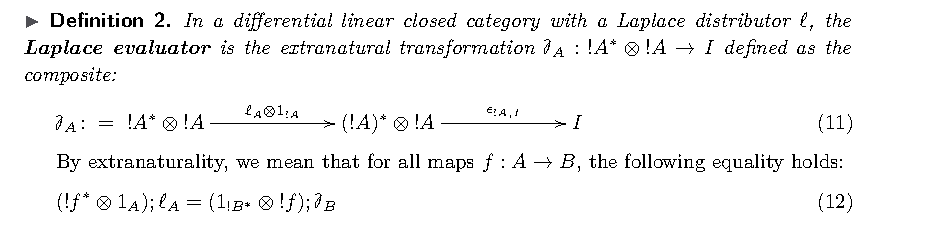
\includegraphics[width=\linewidth]{laplace-evaluator-definition.pdf}\end{center}
\paragraph{Definition3.}
An $I$-exponential map is a map $e:!I\to I$ satisfying the original diagrams:
\begin{center}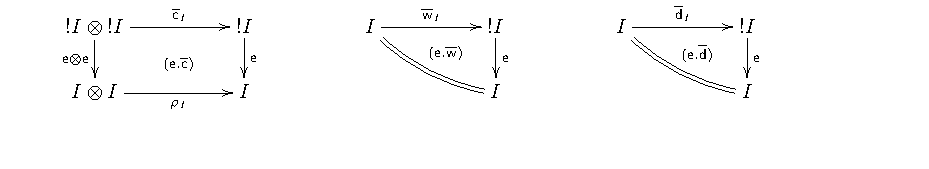
\includegraphics[width=\linewidth]{i-exponential-laws.pdf}\end{center}
% END CONTEXT

% BEGIN SUPPORT: publisher Proposition4 and proof, pp9:9-9:10
\section*{The author constructions}
\paragraph{Proposition4.}
In a differential linear closed category with a Laplace distributor $\ell$, define
\begin{equation}
e^\ell:=!\upsilon_I;\ell_I;\mu_I^*;\upsilon_I^{-1}:!I\to I.\tag{13}
\end{equation}
\paragraph{Proof.}
The key to this proof is using the part from the definition of a monoidal coalgebra
modality[2, Definition1] which says that $d,c,w$ are compatible with $\mu_I$
since they are monoidal transformations. So, by definition,
\begin{equation}
\mu_I;d_I=1_I,\qquad \mu_I;w_I=1_I,\qquad
\mu_I;c_I=\rho_I^{-1};(\mu_I\otimes\mu_I).\tag{14}
\end{equation}
We need the dualized versions
\begin{equation}
d_I^*;\mu_I^*=1_{I^*},\quad
w_I^*;\mu_I^*=1_{I^*},\quad
c_I^*;\mu_I^*=(\mu_I\otimes\mu_I)^*;(\rho_I^{-1})^*.\tag{15}
\end{equation}
First compute $(e.\bar w)$:
\begin{align*}
\bar w_I;e^\ell
&\by{13}\bar w_I;!\upsilon_I;\ell_I;\mu_I^*;\upsilon_I^{-1}\\
&\by{nat.}\bar w_{I^*};\ell_I;\mu_I^*;\upsilon_I^{-1}\\
&\by{\ell.\bar w.1}\upsilon_I;w_I^*;\mu_I^*;\upsilon_I^{-1}
\by{15}\upsilon_I;\upsilon_I^{-1}=1_I.
\end{align*}
Next compute $(e.\bar d)$:
\begin{align*}
\bar d_I;e^\ell
&\by{13}\bar d_I;!\upsilon_I;\ell_I;\mu_I^*;\upsilon_I^{-1}\\
&\by{nat.}\upsilon_I;\bar d_{I^*};\ell_I;\mu_I^*;\upsilon_I^{-1}\\
&\by{\ell.\bar d.1}\upsilon_I;d_I^*;\mu_I^*;\upsilon_I^{-1}
\by{15}\upsilon_I;\upsilon_I^{-1}=1_I.
\end{align*}
Using naturality of $\Theta$ and the following identity, which the authors
leave to the reader to check, we compute $(e.\bar c)$:
\begin{equation}
\Theta_{I,I};(\rho_I^{-1})^*;\upsilon_I^{-1}
=(\upsilon_I^{-1}\otimes\upsilon_I^{-1});\rho_I.\tag{16}
\end{equation}
\begin{align*}
\bar c_I;e^\ell
&\by{13}\bar c_I;!\upsilon_I;\ell_I;\mu_I^*;\upsilon_I^{-1}\\
&\by{nat.}(!\upsilon_I\otimes!\upsilon_I);\bar c_{I^*};\ell_I;\mu_I^*;\upsilon_I^{-1}\\
&\by{\ell.\bar c.1}(!\upsilon_I\otimes!\upsilon_I);(\ell_I\otimes\ell_I);
\Theta_{!I,!I};c_I^*;\mu_I^*;\upsilon_I^{-1}\\
&\by{15}(!\upsilon_I\otimes!\upsilon_I);(\ell_I\otimes\ell_I);
\Theta_{!I,!I};(\mu_I\otimes\mu_I)^*;(\rho_I^{-1})^*;\upsilon_I^{-1}\\
&\by{nat.}(!\upsilon_I\otimes!\upsilon_I);(\ell_I\otimes\ell_I);
(\mu_I^*\otimes\mu_I^*);\Theta_{I,I};(\rho_I^{-1})^*;\upsilon_I^{-1}\\
&\by{16}(!\upsilon_I\otimes!\upsilon_I);(\ell_I\otimes\ell_I);
(\mu_I^*\otimes\mu_I^*);(\upsilon_I^{-1}\otimes\upsilon_I^{-1});\rho_I\\
&\by{13}(e^\ell\otimes e^\ell);\rho_I.
\end{align*}
Therefore $e^\ell$ is an $I$-exponential map. The authors note that
$(\ell.\mu)$ was not needed for this direction.
% END SUPPORT4

% BEGIN SUPPORT5: publisher Proposition5 and proof, pp9:10-9:11
\paragraph{Proposition5.}
If $e:!I\to I$ is an $I$-exponential map, define
$\ell_A^e:!A^*\to(!A)^*$ as the curry of
\begin{equation}
\mu_{A^*,A};!\epsilon_{A,I};e:!A^*\otimes!A\to I.\tag{17}
\end{equation}
In other words, it is the unique map such that
\begin{equation}
(\ell_A^e\otimes1_{!A});\epsilon_{!A,I}
=\mu_{A^*,A};!\epsilon_{A,I};e.\tag{18}
\end{equation}
Then $\ell^e$ is a Laplace distributor; its induced evaluator is(17).
\paragraph{Proof.}
For readability the authors omit subscripts. The key is that evaluation is
monic in its first argument: $(f\otimes1);\epsilon=(g\otimes1);\epsilon$
implies $f=g$. First, naturality:
\begin{align*}
(!f^*\otimes1);(\ell^e\otimes1);\epsilon
&\by{18}(!f^*\otimes1);\mu_{A^*,A};\epsilon;e\\
&\by{nat.}\mu;!(f^*\otimes1);!\epsilon_{A,I};e\\
&\by{10}\mu;!(1\otimes f);!\epsilon;e\\
&\by{nat.}(1\otimes!f);\mu;!\epsilon;e
\by{18}(1\otimes!f);(\ell^e\otimes1);\epsilon\\
&=(\ell^e\otimes1);(1\otimes!f);\epsilon
\by{10}(\ell^e\otimes1);((!f)^*\otimes1);\epsilon.
\end{align*}
Thus $!f^*;\ell^e=\ell^e;(!f)^*$.
The co-structural compatibility relations from[2, Propositions2 and5] are
\begin{align}
(\bar w\otimes1);\mu&=\rho;w;\bar w,\notag\\
(\bar d\otimes1);\mu&=(1\otimes d);\bar d,\notag\\
(\bar c\otimes1);\mu&=(1\otimes1\otimes c);\tau;(\mu\otimes\mu);\bar c.\tag{19}
\end{align}
For $(\ell.\bar w.1)$:
\begin{align*}
(\bar w\otimes1);(\ell^e\otimes1);\epsilon
&\by{18}(\bar w\otimes1);\mu;!\epsilon;e
\by{19}\rho;w;\bar w;!\epsilon;e\\
&\by{nat.}\rho;w;\bar w;e
\by{e.\bar w}\rho;w_A
\by{nat.}(1\otimes w);\rho\\
&\by{7}(1\otimes w);(\upsilon\otimes1);\epsilon
=(\upsilon\otimes1);(1\otimes w);\epsilon\\
&\by{10}(\upsilon\otimes1);(w^*\otimes1);\epsilon.
\end{align*}
Thus $\bar w_{A^*};\ell_A^e=\upsilon_I;w_A^*$.
For $(\ell.\bar d.1)$:
\begin{align*}
(\bar d\otimes1);(\ell^e\otimes1);\epsilon
&\by{18}(\bar d\otimes1);\mu;!\epsilon;e
\by{19}(1\otimes d);\bar d;!\epsilon;e\\
&\by{nat.}(1\otimes d);\epsilon;\bar d;e
\by{e.\bar d}(1\otimes d);\epsilon
\by{10}(d^*\otimes1);\epsilon.
\end{align*}
Thus $\bar d_{A^*};\ell_A^e=d_A^*$.
For $(\ell.\bar c.1)$:
\begin{align*}
(\bar c\otimes1);(\ell^e\otimes1);\epsilon_{!A,I}
&\by{18}(\bar c\otimes1);\mu;!\epsilon;e\\
&\by{19}(1\otimes c);\tau;(\mu\otimes\mu);\bar c;!\epsilon;e\\
&\by{nat.}(1\otimes c);\tau;(\mu\otimes\mu);(!\epsilon\otimes!\epsilon);\bar c;e\\
&\by{e.\bar c}(1\otimes c);\tau;(\mu\otimes\mu);(!\epsilon\otimes!\epsilon);(e\otimes e)\\
&\by{18}(1\otimes c);\tau;((\ell^e\otimes1)\otimes(\ell^e\otimes1));(\epsilon\otimes\epsilon)\\
&\by{nat.}(1\otimes c);((\ell^e\otimes\ell^e)\otimes1);\tau;(\epsilon\otimes\epsilon)\\
&\by{9}((\ell^e\otimes\ell^e)\otimes1);(\Theta\otimes1);(1\otimes c);\epsilon\\
&\by{10}((\ell^e\otimes\ell^e)\otimes1);(\Theta\otimes1);(c^*\otimes1);\epsilon.
\end{align*}
Thus $\bar c_{A^*};\ell_A^e=(\ell_A^e\otimes\ell_A^e);\Theta_{!A,!A};c_A^*$.
Lastly, the monoidal associativity axiom is
\begin{equation}
\alpha;(\mu\otimes1);\mu=(1\otimes\mu);\mu;!\alpha.\tag{20}
\end{equation}
For $(\ell.\mu)$:
\begin{align*}
&(!\nu\otimes1);(\xi\otimes1);((1\multimap\ell^e)\otimes1);(\nu^{-1}\otimes1);\epsilon\\
&\by{8}(!\nu\otimes1);(\xi\otimes1);((1\multimap\ell^e)\otimes1);\alpha;(\epsilon\otimes1);\epsilon\\
&\by{nat.}\alpha;((!\nu\otimes1)\otimes1);((\xi\otimes1)\otimes1);
(((1\multimap\ell^e)\otimes1)\otimes1);(\epsilon\otimes1);\epsilon\\
&\by{5}\alpha;((!\nu\otimes1)\otimes1);((\xi\otimes1)\otimes1);(\epsilon\otimes1);\ell^e;\epsilon\\
&\by{8}\alpha;((!\nu\otimes1)\otimes1);(\mu\otimes1);(!\epsilon\otimes1);\ell^e;\epsilon\\
&\by{nat.}\alpha;(\mu\otimes1);(!(\nu\otimes1)\otimes1);(!\epsilon\otimes1);\ell^e;\epsilon\\
&\by{18}\alpha;(\mu\otimes1);(!(\nu\otimes1)\otimes1);(!\epsilon\otimes1);\mu;!\epsilon;e\\
&\by{nat.}\alpha;(\mu\otimes1);\mu;!((\nu\otimes1)\otimes1));!(\epsilon\otimes1);!\epsilon;e\\
&\by{20}(1\otimes\mu);\mu;!\alpha;!((\nu\otimes1)\otimes1));!(\epsilon\otimes1);!\epsilon;e\\
&\by{8}(1\otimes\mu);\mu;!\epsilon;e
\by{18}(1\otimes\mu);(\ell^e\otimes1);\epsilon\\
&=(\ell^e\otimes1);(1\otimes\mu);\epsilon
\by{10}(\ell^e\otimes1);(\mu^*\otimes1);\epsilon.
\end{align*}
Thus $!\nu_{A,B};\xi_{A,B^*};(1_{!A}\multimap\ell_B^e);\nu_{!A,!B}^{-1}
=\ell_{A\otimes B}^e;\mu_{A,B}^*$.
Therefore $\ell^e$ is a Laplace distributor, and(17) is its induced evaluator.
% END SUPPORT5

% BEGIN STATEMENT: publisher Theorem6, p9:11
\section*{Theorem6}
For a differential linear closed category, there is a bijective correspondence
between Laplace distributors and $I$-exponential maps.
% END STATEMENT

% BEGIN MAIN PROOF: publisher pp9:11-9:12
\paragraph{Proof.}
To show the constructions of Propositions4 and5 are inverses, we must show
$e^{\ell^e}=e$ and $\ell^{e^\ell}=\ell$.
The monoidal unital axiom is
\begin{equation}
(1_{!A}\otimes\mu_I);\mu_{A,I}=\rho_{!A};!(\rho_A^{-1}).\tag{21}
\end{equation}
First:
\begin{align*}
(e^{\ell^e}\otimes1_I);(\upsilon_I\otimes1);\epsilon_{I,I}
&\by{13}(!\upsilon_I\otimes1_I);(\ell_I^e\otimes1_I);(\mu_I^*\otimes1_I);
(\upsilon_I^{-1}\otimes1_I);(\upsilon_I\otimes1);\epsilon_{I,I}\\
&=(!\upsilon_I\otimes1_I);(\ell_I^e\otimes1_I);(\mu_I^*\otimes1_I);\epsilon_{I,I}\\
&\by{10}(!\upsilon_I\otimes1_I);(\ell_I^e\otimes1_I);(1_{(!I)^*}\otimes\mu_I);\epsilon_{!I,I}\\
&=(!\upsilon_I\otimes1_I);(1_{!I^*}\otimes\mu_I);(\ell_I^e\otimes1_{!I});\epsilon_{!I,I}\\
&\by{18}(!\upsilon_I\otimes1_I);(1_{!I^*}\otimes\mu_I);\mu_{I^*,I};!\epsilon_{I^*,I};e\\
&\by{21}(!\upsilon_I\otimes1_I);\rho_{!I^*};!(\rho_{I^*}^{-1});!\epsilon_{I^*,I};e\\
&\by{nat.}\rho_{!I};!\upsilon_I;!(\rho_{I^*}^{-1});!\epsilon_{I^*,I};e\\
&\by{7}\rho_{!I};!\upsilon_I;!\upsilon_I^{-1};e=\rho_{!I};e\\
&\by{nat.}(e\otimes1_I);\rho_I
\by{7}(e\otimes1_I);(\upsilon_I\otimes1);\epsilon_{I,I}.
\end{align*}
So $e^{\ell^e};\upsilon_I=e;\upsilon_I$, and since $\upsilon_I$ is an isomorphism,
$e^{\ell^e}=e$.
On the other hand, the authors leave it as an exercise to check that taking
$B=I$ in $(\ell.\mu)$ gives the following commuting diagram:
\begin{center}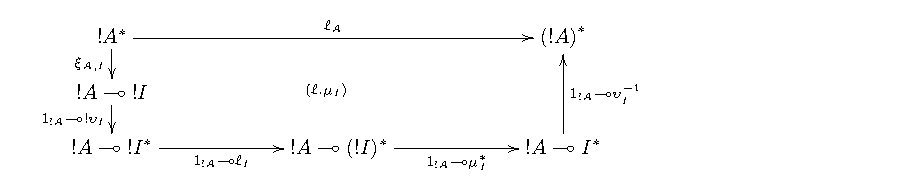
\includegraphics[width=\linewidth]{inverse-laplace-diagram.pdf}\end{center}
From this:
\begin{align*}
(\ell_A^{e^\ell}\otimes1_{!A});\epsilon_{!A,I}
&\by{18}\mu_{A^*,A};!\epsilon_{A,I};e^\ell\\
&\by{13}\mu_{A^*,A};!\epsilon_{A,I};!\upsilon_I;\ell_I;\mu_I^*;\upsilon_I^{-1}\\
&\by{6}(\xi_{A,I}\otimes1_{!A});\epsilon_{!A,!I};!\upsilon_I;\ell_I;\mu_I^*;\upsilon_I^{-1}\\
&\by{5}(\xi_{A,I}\otimes1_{!A});((1_{!A}\multimap!\upsilon_I)\otimes1_{!A});
((1_{!A}\multimap\ell_I)\otimes1_{!A});\\
&\qquad ((1_{!A}\multimap!\upsilon_I)\otimes\mu_I^*);
((1_{!A}\multimap\upsilon_I^{-1})\otimes1_{!A});\epsilon_{!A,I}\\
&\by{\ell.\mu_I}(\ell_A\otimes1_{!A});\epsilon_{!A,I}.
\end{align*}
So $\ell_A^{e^\ell}=\ell_A$.\hfill$\blacktriangleleft$
% END MAIN PROOF

\begin{thebibliography}{99}
\bibitem{source1} R. Blute, T. Ehrhard, and C. Tasson. A convenient differential category. Cahiers de topologie et géométrie différentielle catégoriques, 2012.
\bibitem{source2} R. F. Blute, J. R. B. Cockett, J.-S. P. Lemay, and R. A. G. Seely. Differential categories revisited. Applied Categorical Structures, 2020.
\bibitem{source3} R. F. Blute, J. R. B. Cockett, and R. A. G. Seely. Differential categories. Math. Struct. Comput. Sci., 2006.
\bibitem{source4} F. Breuvart, M. Kerjean, and S. Mirwasser. Unifying graded linear logic and differential operators. In 8th International Conference on Formal Structures for Computation and Deduction, FSCD, 2023.
\bibitem{source5} J. R. B. Cockett and R. A. G. Seely. Weakly distributive categories. Journal of Pure and Applied Algebra, 114(2), 1997.
\bibitem{source6} J. R. B. Cockett and R.A.G. Seely. Proof theory for full intuitionistic linear logic, bilinear logic, and mix categories. Theory and Applications of categories, 3(5), 1997.
\bibitem{source7} J. R. B. Cockett and R.A.G. Seely. Linearly distributive functors. Journal of Pure and Applied Algebra, 143(1-3), 1999.
\bibitem{source8} J.R.B. Cockett and P. V. Srinivasan. Exponential modalities and complementarity (extended abstract). In Kohei Kishida, editor, Proceedings of the Fourth International Conference on Applied Category Theory, Cambridge, United Kingdom, 12-16th July 2021, volume 372 of Electronic Proceedings in Theoretical Computer Science. Open Publishing Association, 2022.
\bibitem{source9} T. Ehrhard. On Köthe Sequence Spaces and Linear Logic. Mathematical Structures in Computer Science, 12(5), 2002.
\bibitem{source10} T. Ehrhard. Finiteness spaces. Mathematical Structures in Computer Science, 15(4), 2005.
\bibitem{source11} T. Ehrhard. An introduction to differential linear logic: proof-nets, models and antiderivatives. Mathematical Structures in Computer Science, 2017.
\bibitem{source12} T. Ehrhard and L. Regnier. Differential interaction nets. Theoretical Computer Science, 364(2), 2006.
\bibitem{source13} A. Fleury and C. Retoré. The mix rule. Mathematical Structures in Computer Science, 4(2), 1994.
\bibitem{source14} R. Gannoun, R. Hachaichi, H. Ouerdiane, and A. Rezgui. Un théorème de dualité entre espaces de fonctions holomorphes à croissance exponentielle. Journal of Functional Analysis, 171(1), 2000.
\bibitem{source15} J.-Y. Girard. Linear Logic. Theoretical Computer Science, 50(1), 1987.
\bibitem{source16} A. Grothendieck. Produits tensoriels topologiques et espaces nucléaires. Memoirs of the AMS, 16, 1966. Publisher: American Mathematical Society.
\bibitem{source17} M. Kerjean. A Logical Account for Linear Partial Differential Equations. In Proceedings of the 33rd Annual ACM/IEEE Symposium on Logic in Computer Science, LICS 2018, Oxford, UK, July 09-12, 2018, 2018.
\bibitem{source18} M. Kerjean and J.-S. P. Lemay. Taylor Expansion as a Monad in Models of DiLL. In 2023 38th Annual ACM/IEEE Symposium on Logic in Computer Science (LICS), 2023.
\bibitem{source19} O. Laurent. Etude de la polarisation en logique. Thèse de Doctorat, Université Aix-Marseille II, March 2002.
\bibitem{source20} J.-S. P. Lemay. Exponential functions in cartesian differential categories. Applied Categorical Structures, 29, 2021.
\bibitem{source21} J.-S. P. Lemay and J.-B. Vienney. Graded differential categories and graded differential linear logic. In Mathematical Foundations of Programming Semantics, 2023.
\bibitem{source22} P.-A. Melliès. Categorical semantics of linear logic. Société Mathématique de France, 2008.
\bibitem{source23} C.-H. L. Ong. Quantitative semantics of the lambda calculus: Some generalisations of the relational model. In 31st Annual ACM/IEEE Symposium on Logic in Computer Science (LICS), 2017.
\end{thebibliography}
\end{document}
